%---------- Inleiding ---------------------------------------------------------

\section{Introductie}%
\label{sec:introductie}

Bij volwassenen wordt een sedentaire levensstijl geassocieerd met schadelijke gevolgen voor de volgende gezondheidskwesties: sterfte in het algemeen, sterfte door hart- en vaatziekten en kanker, het voorkomen van hart- en vaatziekten, diabetes type 2 en kanker \autocite{Bull2020}. Het is dus van groot belang dat voldoende beweging een prioriteit is.

Daarnaast gaan verminderde fysieke activiteit ook gepaard met meer depressie-, angst- en \linebreak stresssymptomen \autocite{Stanton2020}.

Volgens \textcite{Bull2020} moeten volwassenen tussen de 18 en 64 jaar oud, wekelijks 150 à 300 minuten sporten met gemiddelde intensiteit, of 75 à 150 minuten met krachtige intensiteit. Voor mensen met een beperking worden dezelfde hoeveelheden sport aangeraden, hoewel daar mogelijks samen met een medisch verantwoordelijke bekeken moet worden in welke mate dit mogelijk is, afhankelijk van de beperking. Voor zwangere of net bevallen vrouwen wordt er minstens 150 minuten per week, met gemiddelde intensiteit, aangeraden.

Wereldwijd beschouwt \autocite{Hallal2012} 31,1\% van de bevolking als inactief. Dit wil zeggen dat, op het moment van onderzoek, bijna een derde van de volwassen wereldbevolking de vooropgestelde aanbevelingen van ``World Health Organization'' (WHO), beschreven door \autocite{Bull2020} niet haalt. Voor Europa ligt deze waarde zelfs op 34,8\% en zoals op Figuur \ref{fig:inactivity} gezien, ligt België nog een stuk boven de gemiddelde Europese waarde.

\begin{figure}[t]
    \caption{Fysieke inactiviteit volwassenen (15+) wereldwijd, bij mannen (A) en vrouwen (B) \autocite{Bull2020}}
    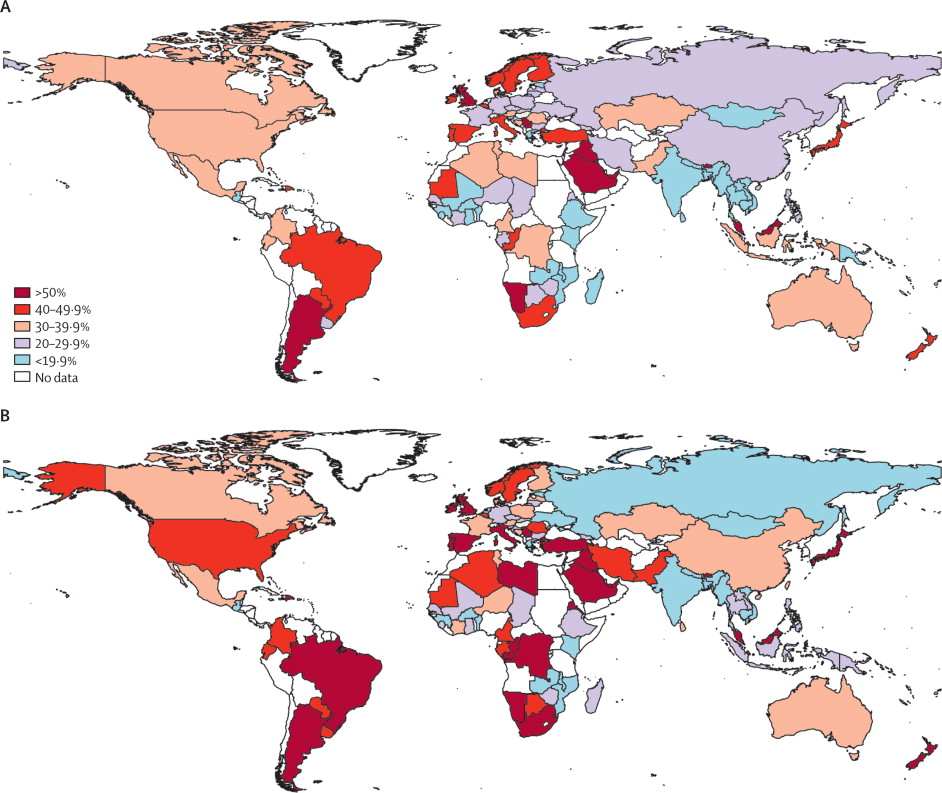
\includegraphics[width=0.5\textwidth]{Inactiviteit}
    \label{fig:inactivity}
\end{figure}

Om deze problematiek te proberen verhelpen, zal een sportplatform ontwikkeld worden. Deze paper onderzoekt hoe gamification hierbij kan helpen. Gamification is in de literatuur beschreven als het gebruiken van spelelementen in een context die niet aan een spel gerelateerd is \autocite{Gaalen2020}.

In de literatuurstudie zal allereerst het belang van beweging gekaderd worden. Ten tweede zal het concept van gamification uiteengezet worden. Daarna zullen de populairste technieken, sociale aspecten en de invloed van gamification op het gedrag en de psychologische staat van gebruikers besproken worden. Dan zal het effect dat beweging en een gezonde levensstijl heeft op productiviteit geïllustreerd worden. Ten slotte wordt er gekeken naar bestaande sportapplicaties en -platformen, en beschreven welke vormen van gamification daar in voorkomen.

Nadien zal in de methodologie worden uiteengezet welke stappen er nodig zijn om tot het sportplatform te komen dat, door middel van gamification, werknemers van \textbf{bedrijfX} en \textbf{bedrijfY} motiveert om meer te sporten.

Uiteindelijk kunnen de conclusies van het onderzoek teruggevonden worden.


% Waarover zal je bachelorproef gaan? Introduceer het thema en zorg dat volgende zaken zeker duidelijk aanwezig zijn: de doelgroep

% De doelgroep moet ook concreet en duidelijk zijn, dus geen algemene of vaag gedefinieerde groepen zoals \emph{bedrijven}, \emph{developers}, \emph{Vlamingen}, enz. Je richt je in elk geval op it-professionals, een bachelorproef is geen populariserende tekst. Eén specifiek bedrijf (die te maken hebben met een concrete probleemsituatie) is dus beter dan \emph{bedrijven} in het algemeen.

%---------- Stand van zaken ---------------------------------------------------

\section{Literatuurstudie}%
\label{sec:state-of-the-art}

\subsection{Belang van beweging}

\subsection{Gamification}

Volgens \textcite{Deterding2011} is gamification te beschrijven als het gebruiken van speldesignelementen in een niet-spelgerelateerde context. Gamification bestaat uit drie hoofdonderdelen: de gebruikte techniek, de psychologische uitkomsten en de verdere invloed op het gedrag \autocite{Hamari2014}. Daarnaast zijn sociale aspecten ook essentieel: door het ontstaan van een competitie streven mensen ernaar erkenning te ontvangen \autocite{Hamari2013}.

\subsubsection{Populairste technieken}
Volgens \textcite{Hamari2014} zijn punten, scoreborden en vooropgestelde uitdagingen de drie meest voorkomende technieken. Daarnaast komen ook het gebruik van levels \autocite{Dong2012}, beloningen \autocite{Flatla2011} en een overzicht van vooruitgang of het bekomen van badges \autocite{Li2012} veelvuldig voor.

\subsubsection{Sociale aspecten van gamification}
Sociale invloed verwijst naar de perceptie van een individu over het belang dat anderen hechten aan een bepaald doelgedrag en of ze verwachten dat iemand dat gedrag zal vertonen \autocite{Ajzen1991}.

Herkenning beschrijft de sociale feedback die gebruikers krijgen op hun gedrag \autocite{Cheung2011}. \textcite{Hamari2013} suggereren dat het ontvangen van erkenning, een bepaalde bereidheid creëert om anderen binnen eenzelfde dienst wederzijds te erkennen, wat de sociale interactie verder bevordert.

Beide aspecten zijn belangrijk om in acht te nemen wanneer gamification geïmplementeerd wordt. Het is volgens \textcite{Preece2001} namelijk zo dat een service positiever wordt ervaren wanneer het een gevoel van erkenning door andere gebruikers oplevert. Dit zal er op zijn beurt voor zorgen dat de houding van de gebruiker ten opzichte van de dienst positief beïnvloed wordt.

\subsubsection{Invloed van gamification}
Op dit moment is vooral de invloed die gamification heeft op het gedrag van de gebruiker onderzocht. Wanneer psychologische gevolgen ook bevraagd zijn, wordt er vooral gefocust op motivatie, attitude en plezier \autocite{Hamari2014}. Studies van \textcite{Hamari2013a} hebben aangetoond dat de resultaten van gamification mogelijks niet voor alle gebruikers op lange termijn doeltreffend zijn.

\subsection{Beweging en productiviteit}



\subsection{Gamification in bestaande sportapplicaties}


% Zijn er al gelijkaardige onderzoeken gevoerd? Wat concluderen ze? Wat is het verschil met jouw onderzoek?


%---------- Methodologie ------------------------------------------------------
\section{Methodologie}%
\label{sec:methodologie}

Het onderzoek zal beginnen met een literatuurstudie over gamification. Hierbij is het belangrijk om technieken te identificeren die van toepassing zijn op deze specifieke casus. De resultaten hiervan kunnen gebruikt worden in de volgende fase.

Deze volgende fase bestaat uit een bevraging bij IT-werknemers van \textbf{enkele} Gentse bedrijven. De bedoeling hiervan is enerzijds achterhalen in welke mate sport en beweging een rol speelt in hun dagelijkse leven op het moment van het interview, en anderzijds te weten komen in welke mate en op welke manieren deze werknemers gestimuleerd kunnen worden om meer te gaan sporten, aan de hand van een competitief sportplatform. Hier kan ook de theorie die verkregen is uit de literatuurstudie getoetst worden.

Steunend op de bekomen resultaten uit zowel de literatuurstudie als de analyse van de gebruikersinterviews, zal dan een applicatie ontwikkeld worden. Het platform zal bestaan in de vorm van een responsive \href{https://react.dev/}{React}-website, geschreven in \href{https://www.typescriptlang.org/}{TypeScript}, waarin sportgegevens van deelnemende werknemers worden verzameld aan de hand van applicaties en hun ''Application Programming Interface'' (API) zoals \href{https://developers.strava.com/}{Strava}, \href{https://dev.fitbit.com/}{Fitbit} en \href{https://developer.garmin.com/gc-developer-program/overview/}{Garmin Connect}. Deze gegevens zullen in combinatie met gamification gebruikt worden om een competitie tussen de deelnemende bedrijven op te zetten.

Deze POC zal dan dienen om de hypotheses te toetsen: heeft het competitief sportplatform, dat gebruik maakt van gamification, een positieve invloed op het sportgedrag van werknemers in een sedentaire job? Om deze vraag te beantwoorden zullen opnieuw gebruikersinterviews plaatsvinden, met dezelfde personen die voor aanvang van de ontwikkelingsfase geïnterviewd zijn en die voor een periode van enkele weken deze POC hebben kunnen gebruiken. Een grondige analyse van de sportgegevens op het platform en de antwoorden van deze ondervraging, leiden tot de conclusie van dit onderzoek.

% Je beschrijft ook al welke tools (hardware, software, diensten, \ldots) je denkt hiervoor te gebruiken of te ontwikkelen.

% Probeer ook een tijdschatting te maken. Hoe lang zal je met elke fase van je onderzoek bezig zijn en wat zijn de concrete \emph{deliverables} in elke fase?

%---------- Verwachte resultaten ----------------------------------------------
\section{Verwacht resultaat}%
\label{sec:verwachte_resultaten}

De verworven kennis geeft momenteel aan dat een sportplatform met implementatie van gamification wel degelijk een positieve invloed zal hebben op het sportgedrag van gebruikers. Deze conclusie ... onder voorwaarde dat er voldoende aandacht besteed wordt aan het sociale aspect van gamification en de gebruikers ook een persoonlijke ontwikkeling kunnen opmerken op het platform.

% TODO: iets over productiviteit

% Hier beschrijf je welke resultaten je verwacht. Als je metingen en simulaties uitvoert, kan je hier al mock-ups maken van de grafieken samen met de verwachte conclusies. Benoem zeker al je assen en de onderdelen van de grafiek die je gaat gebruiken. Dit zorgt ervoor dat je concreet weet welk soort data je moet verzamelen en hoe je die moet meten.

% Wat heeft de doelgroep van je onderzoek aan het resultaat? Op welke manier zorgt jouw bachelorproef voor een meerwaarde?

% Hier beschrijf je wat je verwacht uit je onderzoek, met de motivatie waarom. Het is \textbf{niet} erg indien uit je onderzoek andere resultaten en conclusies vloeien dan dat je hier beschrijft: het is dan juist interessant om te onderzoeken waarom jouw hypothesen niet overeenkomen met de resultaten.

